\documentclass[12pt]{article}
\usepackage{graphicx}
\usepackage{subcaption}
\usepackage{mwe}
\usepackage{amsmath}
\usepackage{mathtools}
\usepackage[]{mcode}
%\usepackage{lingmacros}
%\usepackage{tree-dvips}
%\usepackage{blindtext}
%\usepackage[utf8]{inputenc}

\newcommand{\norm}[1]{\left\lVert#1\right\rVert}
\newcommand{\abs}[1]{\left|#1\right|}

\begin{document}

\title{CMSC 426 - P4}
\author{Gudjon Einar Magnusson}

\maketitle

\section{Introduction}

The goal of this project is to track the precise boundary of an object of interest through a sequence of frames. The object, camera and background may or may not be moving. The only assumption is that the precise shape and location of the object is given for the first frame and that the object will only make small movements from one frame to the next.

\section{Select the Object of Interest}

\begin{figure}
	\centering
    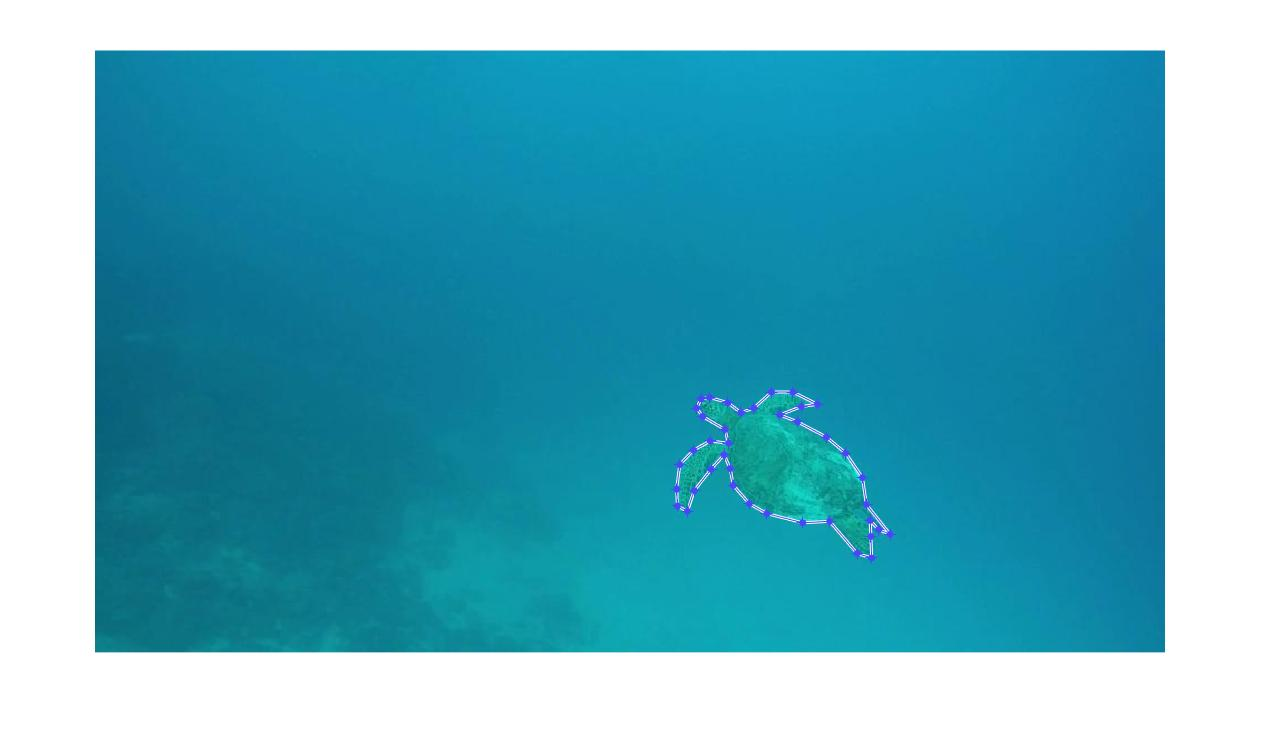
\includegraphics[width=0.6\linewidth]{img/video1_mask1}
    \caption{Capturing the region of interest using a hand drawn polygon}
    \label{fig_roi1}
\end{figure}

To be able to track an object of interest, we first need to know what that object is. To do this the boundary of the object needs to be marked on the first frame. This is done using the \textit{roipoly} Matlab function. It allows the user to draw an arbitrary polygon on top of an image and returns that polygon as a binary mask. Figure \ref{fig_roi1} shows an example of how the polygon is drawn to track a turtle in a video.

The user supplied mask does not need to be pixel perfect, it just needs to be good enough to supply sufficient examples of foreground and background pixels. The mask is used to generate a classifier that is then used to refine the mask.


\section{Color classifier}

A color classifier is generated taking the mean of all the pixels inside the foreground mask and the mean of all pixels on the outside. This gives two class centroids, $\mu_{FG}$ and $\mu_{BG}$. Each pixel $x_i$ can now be classified using the formula 

\[
1 - \frac{\norm{x_i - \mu_{FG}}}{\norm{x_i - \mu_{FG}}+\norm{x_i - \mu_{BG}}}
\]

This gives a new gray scale mask where the intensity of each pixel represents the probability that the pixel belongs to the foreground.

\section{Small Overlapping Windows}

Within the object we want to track, there may be a variety of colors and textures and the background may also be variable. Because of this it is extremely challenging to define a single, global classifier. \cite{snapcut} proposes a method that splits the object boundary into multiple, overlapping windows and defines a color classifier separately for each window. This way there is much less variability for the classifier to deal with.

This implementation uses a simplified version of this window technique. The bounding box of the region of interest is covered in square regions (typically of size 10 - 30 pixels). Each square is then padded by half its size so it overlaps its neighbors, this ensures that every pixel in the region is covered by multiple windows.

Using the object mask that we have defined, a color classifier is generated for each window using the region of the image that it covers. The mask is refined by classifying each pixel in a region using its classifier. The overlap is resolved by picking the maximum response for each pixel.

\begin{figure}
    \begin{subfigure}[t]{.49\textwidth}
        \centering
        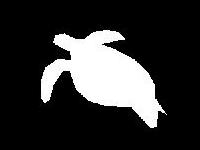
\includegraphics[width=\linewidth]{img/mask_user}
        \caption{Object mask defined by user}
        \label{fig_mask_refine_a}
    \end{subfigure}\hfill
    \begin{subfigure}[t]{.49\textwidth}
        \centering
        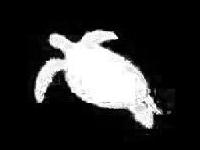
\includegraphics[width=\linewidth]{img/mask_refined}
        \caption{Refined object mask using color classifiers}
        \label{fig_mask_refine_b}
    \end{subfigure}
    \label{fig_mask_refine}
\end{figure}

On problem with this approach is that some windows don't overlap the boundary that we are trying to track, or just overlap by a few pixels. This makes it either impossible to define a classifier or it might be a bad classifier because of the small sample size. To handle this windows are ignored if the ratio between foreground and background samples is too high or low. In the current implementation the window is ignored if either class covers more than 90\% of the samples. That ratio can be tweaked depending on the window size.


\section{Propagate To Next Frame}

In order to track a moving object we need some way to propagate the results from one frame to the next and be able to adapt to changes in shape and color.

\subsection{The Naive Approach}

One simple way to do this is to keep the window size large enough that the boundary will not move across it in one frame. On frame $i$ we setup the windows and define the classifiers. On frame $i+1$ we use the classifiers again with the windows in the same location and use that result to recalculate the window locations and define new classifiers. This works if the windows are large, the movement is small and the color classifiers can be trusted completely.

If to much trust is put into the color classifier alone the color can creep away from the original object after a few frames. Figure \ref{fig_color_creep} shows how the color classification can get out of hand.

\begin{figure}
	\centering
    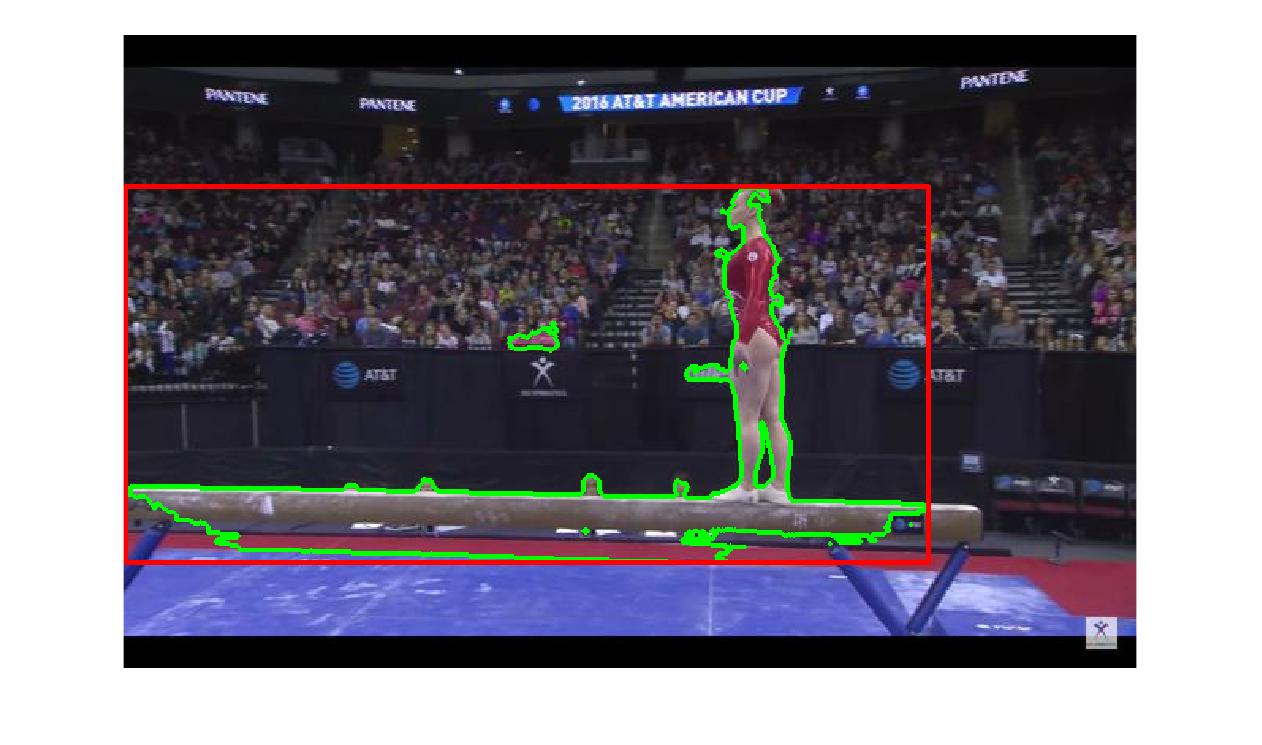
\includegraphics[width=0.6\linewidth]{img/color_creep}
    \caption{Object boundary after 200 frames of naive mask propagation}
    \label{fig_color_creep}
\end{figure}

\subsection{The Better Approach}

I spent too long trying to get this to work without using optical flow because I was having some technical issues. I see now that that is the only way to track the shape and avoid the color creep. 

\begin{thebibliography}{9}

\bibitem{snapcut}
  Xue Bai, Jue Wang, David Simons, Guillermo Sapiro
  \emph{Video snapcut: robust video object cutout using localized classifiers},
  ACM Transactions on Graphics (TOG),
  2009/7/27

\end{thebibliography}

\end{document}